\documentclass[tikz,border=8pt]{standalone}
\usepackage{tikz}
\usepackage{tkz-euclide}
\usepackage{amsmath, amssymb}

\begin{document}

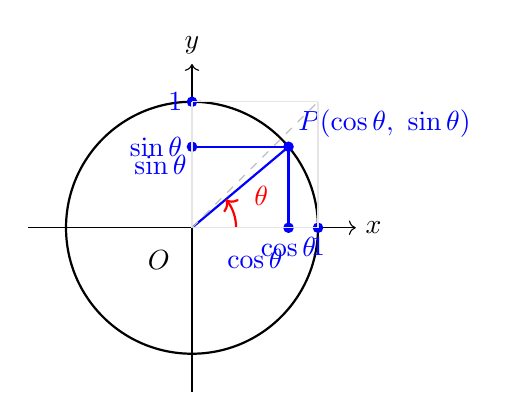
\begin{tikzpicture}[scale=1.6]

  % ---- Circunferencia unitaria ----
  \draw[thick] (0,0) circle (1);
  \draw[->] (-1.3,0) -- (1.3,0) node[right] {$x$};
  \draw[->] (0,-1.3) -- (0,1.3) node[above] {$y$};
  \node[below left] at (-0.1,-0.1) {$O$};

  % ---- Ángulo θ en primer cuadrante ----
  \coordinate (A) at (1,0);
  \coordinate (B) at ({cos(40)},{sin(40)});
  \draw[thick, blue] (0,0) -- (B);
  \draw[thick, blue] (B) -- (B |- 0,0);  % proyección en x
  \draw[thick, blue] (B) -- (0,0 |- B);  % proyección en y

  % ---- Arco del ángulo ----
  \draw[->, thick, red] (0.35,0) arc (0:40:0.35);
  \node[red] at (0.55,0.25) {$\theta$};

  % ---- Puntos y etiquetas ----
  \fill[blue] (B) circle (1.2pt) node[above right] {$P(\cos\theta,\ \sin\theta)$};
  \fill[blue] (B |- 0,0) circle (1.2pt) node[below] {$\cos\theta$};
  \fill[blue] (0,0 |- B) circle (1.2pt) node[left] {$\sin\theta$};
  \fill[blue] (1,0) circle (1.2pt) node[below] {$1$};
  \fill[blue] (0,1) circle (1.2pt) node[left] {$1$};

  % ---- Cuadrante y cuadrícula sutil ----
  \draw[gray!20] (0,0) grid (1,1);
  \draw[gray!50, dashed] (0,0) -- (1,1);

  % ---- Etiquetas de funciones trigonométricas ----
  \node[blue] at (0.5,-0.25) {$\cos\theta$};
  \node[blue] at (-0.25,0.5) {$\sin\theta$};

\end{tikzpicture}

\end{document}
